This chapter translates the technology selections of Chapter~3 into a concrete system design and reports the implementation outcomes obtained on Solana Devnet. The prototype has not been deployed on Mainnet Beta, has not undergone a third-party security audit, and has not been subjected to a large-scale user study; the results reported in this chapter should be read in that light.

\section{Architecture}
\label{section:4.1}

FreelanceChain adopts a \textbf{blockchain-centric three-layer architecture}. The \textbf{presentation layer} is a Next.js application that renders the UI, manages client-side state, and translates user actions into Solana transactions; it neither holds funds nor enforces business rules. The \textbf{business-logic layer} is the Anchor program deployed to Solana, comprising eighteen modules organized into five groups: \emph{Core} (\emph{job\_management}, \emph{token\_escrow}, \emph{milestone}), \emph{Identity \& Privacy} (\emph{kyc}, \emph{did}, \emph{sybil\_resistance}, \emph{zk\_proofs}), \emph{Reputation \& AI} (\emph{sbt\_reputation}, \emph{ai\_oracle}), \emph{Governance} (\emph{dao\_governance}, \emph{governance\_token}, \emph{referral}), and \emph{Account Security} (\emph{social\_recovery}, \emph{account\_abstraction}). This layer is the sole authoritative enforcer of all platform rules. The \textbf{data layer} is hybrid: the Solana blockchain holds transactional state in PDA accounts, \gls{ipfs} holds large documents and metadata, and browser \emph{localStorage} caches session-scoped data (KYC status hint, profile data, referral source) to minimize redundant on-chain reads. The \emph{localStorage} cache is never authoritative: every security-relevant decision re-derives state from the chain.

An optional \textbf{observability sidecar} (Section~\ref{section:4.7}) sits outside the three layers above. It polls the public Solana RPC, decodes the program's PDA state, and exposes Prometheus metrics consumed by Grafana. Because it is read-only and reads exclusively public ledger data, it neither introduces a new trust assumption nor is required for the dApp to function; anyone may run their own instance to obtain an independent view of program health.

\begin{figure}[H]
    \centering
    \includegraphics[width=0.75\textwidth]{system_layer.png}
    \caption{Three-layer system architecture.}
    \label{fig:architecture}
\end{figure}

\begin{figure}[H]
    \centering
    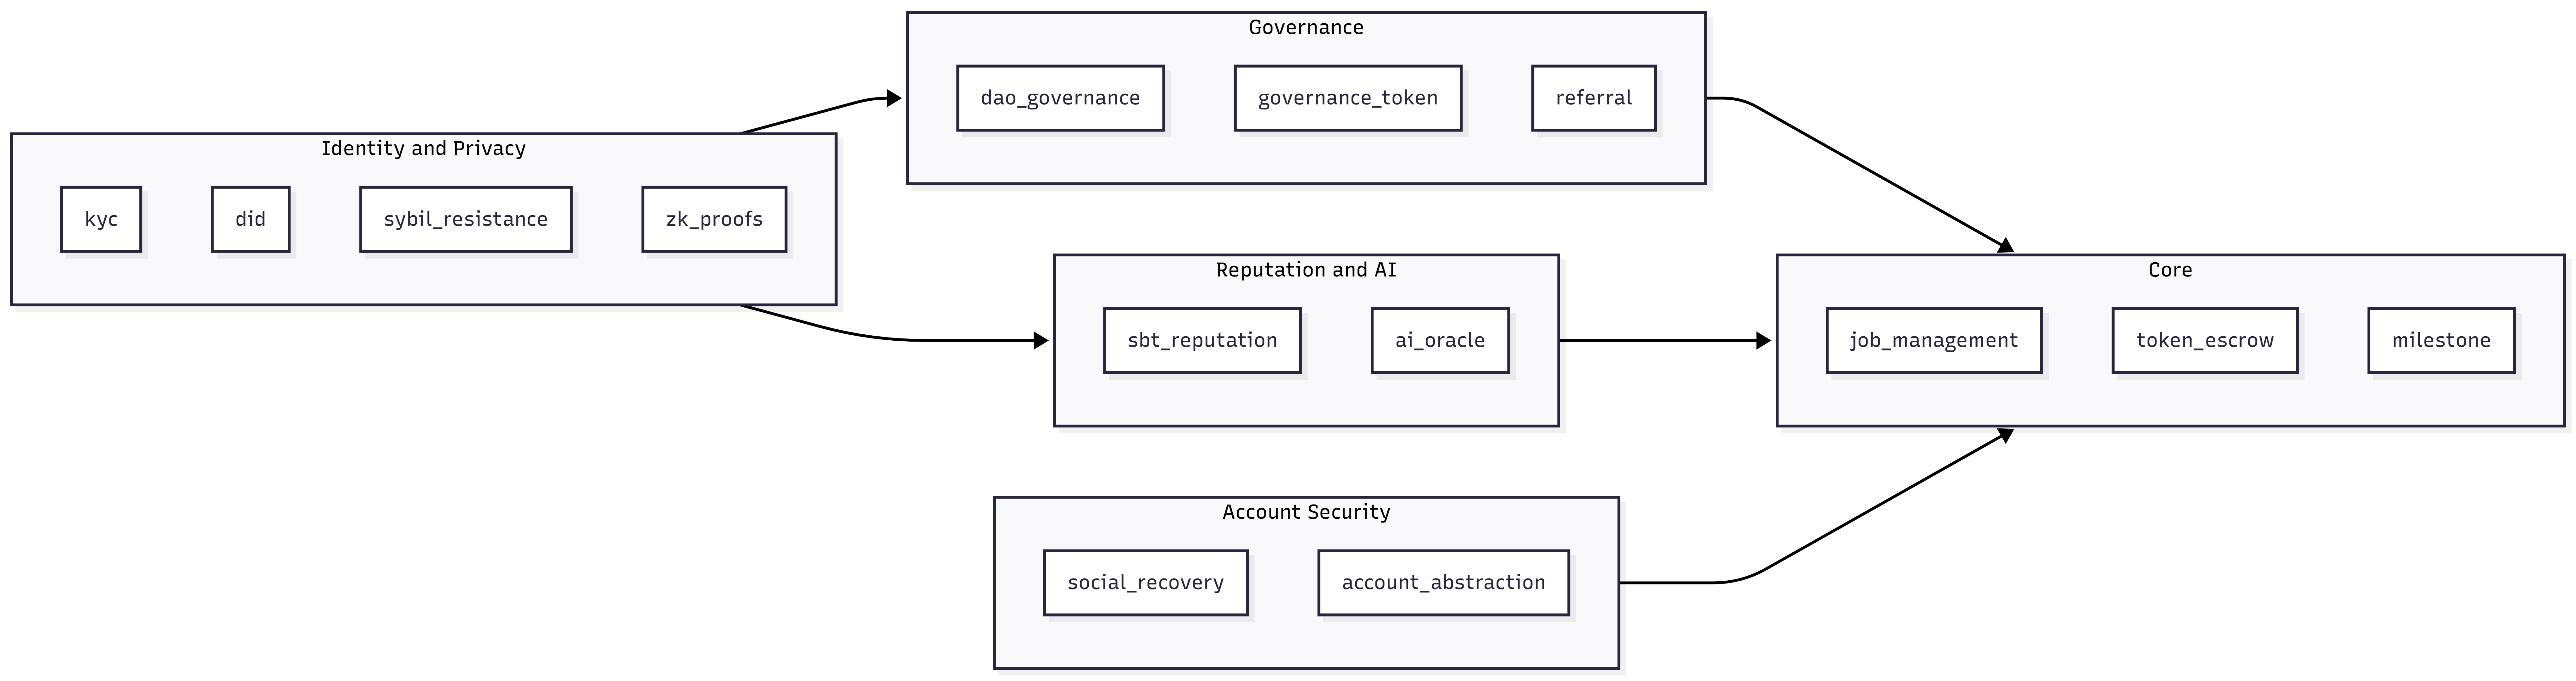
\includegraphics[width=1.0\textwidth]{module_map.png}
    \caption{Smart-contract module dependency map.}
    \label{fig:module_map}
\end{figure}


\section{Detailed Design}
\label{section:4.2}

\subsection{User Interface}

The user interface targets desktop browsers while retaining a responsive layout for narrower screens. Its visual language follows a crypto-terminal style so that blockchain actions, wallet state, and transaction feedback remain visually distinct from ordinary content. Screenshots of the principal flows (job creation, bid submission, escrow funding, release/dispute, KYC, SBT minting, and DAO voting) are reproduced in Figures~\ref{fig:demo_create_job}--\ref{fig:demo_dao_vote} of Section~\ref{section:4.5}.

\begin{figure}[H]
    \centering
    \includegraphics[width=1.0\textwidth]{screen1.png}
    \caption{Job detail page (representative screen).}
    \label{fig:jobdetail}
\end{figure}


\subsection{Account Schemas}
\label{subsection:4.2.2}

This subsection enumerates the principal Program-Derived Account (PDA) types of the Anchor program. For each account the relevant fields, types, seed derivation, the instructions that create/update it, and the writer authority are tabulated. The tables reflect the source structures in \emph{programs/freelance-marketplace/src/}; trivial Anchor fields (\emph{bump}, sequence counters) are listed but not further commented.

\begin{table}[H]
\centering
\caption{JobAccount (Job in source). Seed: \emph{[b"job", client, job\_id\_le]}. Owner: client (signs creation). Writers: client via lifecycle instructions.}
\label{table:pda_job}
\small
\begin{tabular}{|l|l|p{6.5cm}|}
\hline
\textbf{Field} & \textbf{Type} & \textbf{Notes / instructions that mutate it} \\ \hline
\emph{client} & Pubkey & Set by \emph{create\_job}; immutable. \\ \hline
\emph{title} & String(100) & \emph{create\_job}. \\ \hline
\emph{description} & String(500) & \emph{create\_job}. \\ \hline
\emph{budget} & u64 (lamports) & \emph{create\_job}; upper bound on aggregate escrow. \\ \hline
\emph{metadata\_uri} & String(200) & IPFS CID; \emph{create\_job}. \\ \hline
\emph{token\_mint} & \emph{Option\textless{}Pubkey\textgreater{}} & \emph{None} = SOL, \emph{Some} = SPL mint. \\ \hline
\emph{status} & JobStatus enum & State machine of Section~\ref{subsection:4.2.3}. \\ \hline
\emph{selected\_freelancer} & \emph{Option\textless{}Pubkey\textgreater{}} & Set by \emph{select\_bid}. \\ \hline
\emph{escrow\_amount} & u64 & Tracked across deposit/release. \\ \hline
\emph{bid\_count}, timestamps, \emph{bump} & u32, i64, u8 & Bookkeeping fields. \\ \hline
\end{tabular}
\end{table}

\begin{table}[H]
\centering
\caption{BidAccount (Bid). Seed: \emph{[b"bid", job, freelancer]} -- one bid per (job, freelancer) pair. Owner: freelancer (signs creation).}
\label{table:pda_bid}
\small
\begin{tabular}{|l|l|p{6.5cm}|}
\hline
\textbf{Field} & \textbf{Type} & \textbf{Notes / mutators} \\ \hline
\emph{job}, \emph{freelancer} & Pubkey & Pinned at \emph{submit\_bid}. \\ \hline
\emph{proposed\_budget} & u64 & Lamports proposed by freelancer. \\ \hline
\emph{proposal} & String(500) & Free-text proposal body. \\ \hline
\emph{timeline\_days} & u16 & Promised delivery window. \\ \hline
\emph{cv\_uri} & String(200) & IPFS CID, may be empty. \\ \hline
\emph{status} & BidStatus enum & Pending/Accepted/Rejected; mutated by \emph{select\_bid}. \\ \hline
\emph{created\_at}, \emph{bump} & i64, u8 & \\ \hline
\end{tabular}
\end{table}

\begin{table}[H]
\centering
\caption{EscrowAccount (Escrow). Seed: \emph{[b"escrow", job]} -- single escrow per job. Writers: client (deposit), program (release/dispute), arbitrators (dispute resolution).}
\label{table:pda_escrow}
\small
\begin{tabular}{|l|l|p{6.5cm}|}
\hline
\textbf{Field} & \textbf{Type} & \textbf{Notes / mutators} \\ \hline
\emph{job}, \emph{client}, \emph{freelancer} & Pubkey & Bound at \emph{deposit\_token\_escrow}. \\ \hline
\emph{amount} & u64 & Funds locked in PDA-controlled balance. \\ \hline
\emph{locked}, \emph{released}, \emph{disputed} & bool & Encode escrow state machine of Section~\ref{subsection:4.2.3}. \\ \hline
\emph{created\_at}, \emph{bump} & i64, u8 & \\ \hline
\end{tabular}
\end{table}

\begin{table}[H]
\centering
\caption{MilestoneAccount and MilestoneEscrow. Seeds: \emph{[b"milestone", job, index]} and \emph{[b"ms-escrow", milestone]}. Writers: client for create/fund/approve, freelancer for submission.}
\label{table:pda_milestone}
\small
\begin{tabular}{|l|l|p{6.5cm}|}
\hline
\textbf{Field} & \textbf{Type} & \textbf{Notes / mutators} \\ \hline
\emph{job}, \emph{milestone\_index} & Pubkey, u8 & Pinned at \emph{create\_milestone}. \\ \hline
\emph{title}, \emph{description} & String & Up to 100/500 chars. \\ \hline
\emph{amount} & u64 & Validated against job budget on funding. \\ \hline
\emph{status} & MilestoneStatus & Created $\to$ Funded $\to$ Submitted $\to$ Approved/Rejected/Disputed. \\ \hline
\emph{deliverable\_uri} & String(200) & IPFS CID set on submission. \\ \hline
\emph{submitted\_at}, \emph{approved\_at} & \emph{Option\textless{}i64\textgreater{}} & Timestamps. \\ \hline
\multicolumn{3}{|l|}{\emph{Companion} MilestoneEscrow \emph{(seed} \emph{[b"ms-escrow", milestone]}\emph{): mirrors lock/release flags above.}} \\ \hline
\end{tabular}
\end{table}

\begin{table}[H]
\centering
\caption{KycRecord. Seed: \emph{[b"kyc", user]}. Writers: user only (via \emph{submit\_kyc}/\emph{finalize\_kyc}/\emph{reset\_kyc}).}
\label{table:pda_kyc}
\small
\begin{tabular}{|l|l|p{6.5cm}|}
\hline
\textbf{Field} & \textbf{Type} & \textbf{Notes / mutators} \\ \hline
\emph{authority} & Pubkey & The user owning the record. \\ \hline
\emph{status} & KycStatus & Pending / Verified / Rejected. \\ \hline
\emph{id\_type} & IdType enum & National ID / Passport / Driver's licence. \\ \hline
\emph{submitted\_at}, \emph{verified\_at} & i64 & Set by submit/finalize. \\ \hline
\emph{verification\_hash} & \emph{[u8;\,32]} & SHA-256 of (quantized descriptor $\|$ id\_type $\|$ wallet). \\ \hline
\end{tabular}
\end{table}

\noindent The implementation also exposes a \emph{face\_distance\_bp} parameter (u32) that the smart contract uses to gate finalization: only the integer outcome and the hash are persisted, never the raw 128-dimensional descriptor itself.

\begin{table}[H]
\centering
\caption{ReputationSbtAccount (ReputationSBT). Seed: \emph{[b"sbt", reviewee, sbt\_index\_le]}. Writer: rater via \emph{mint\_reputation\_sbt}; revocation by the original rater only via \emph{revoke\_sbt}.}
\label{table:pda_sbt}
\small
\begin{tabular}{|l|l|p{6.5cm}|}
\hline
\textbf{Field} & \textbf{Type} & \textbf{Notes / mutators} \\ \hline
\emph{user}, \emph{job}, \emph{rater} & Pubkey & Bound at mint, immutable thereafter. \\ \hline
\emph{rating} & u8 & Range $[1,5]$ enforced on-chain. \\ \hline
\emph{comment} & String(200) & Optional review text. \\ \hline
\emph{job\_amount} & u64 & Captured at mint for context. \\ \hline
\emph{verification\_hash} & \emph{[u8;\,32]} & SHA-256(job $\|$ reviewer $\|$ rating $\|$ ts). \\ \hline
\emph{sbt\_index} & u32 & Sequential per recipient (read from companion counter PDA). \\ \hline
\emph{revoked} & bool & Only the original rater may set. \\ \hline
\end{tabular}
\end{table}

\begin{table}[H]
\centering
\caption{GovernanceProposal (Proposal). Seed: \emph{[b"proposal", proposal\_id\_le]}. Writers: proposer for create; the program for finalize/execute; voters write companion DAOVote PDAs (seed \emph{[b"dao-vote", proposal, voter]}).}
\label{table:pda_proposal}
\small
\begin{tabular}{|l|l|p{6.5cm}|}
\hline
\textbf{Field} & \textbf{Type} & \textbf{Notes / mutators} \\ \hline
\emph{id}, \emph{proposer} & u64, Pubkey & Pinned at \emph{create\_proposal}. \\ \hline
\emph{title}, \emph{description\_uri} & String & 100/200 chars; IPFS CID for body. \\ \hline
\emph{proposal\_type} & u8 & Encodes ParameterChange, FundAllocation, FeatureVote, GovernanceUpgrade, EmergencyAction. \\ \hline
\emph{status} & u8 & Active / Passed / Rejected / Executed. \\ \hline
\emph{votes\_for}, \emph{votes\_against} & u64 & Weighted by token balance $\times$ SBT multiplier. \\ \hline
\emph{stake\_amount} & u64 & Anti-spam stake (refundable on pass). \\ \hline
\emph{created\_at}, \emph{voting\_ends\_at} & i64 & Period derived from DAO config. \\ \hline
\emph{executed} & bool & Set by \emph{execute\_proposal} once. \\ \hline
\end{tabular}
\end{table}

\noindent Additional companion accounts (SbtCounterAccount, DAOConfig, DAOVote, Dispute, VoteRecord, Reputation, Review, Referral, RecoveryConfig, ZkCredential, AiVerification) follow the same layout pattern: a strongly typed Anchor struct, deterministic seeds rooted at a semantically meaningful key, and writer constraints expressed via Anchor's \emph{has\_one}, \emph{constraint}, and \emph{signer} attributes.

\subsection{State Machines: Job and Escrow Lifecycles}
\label{subsection:4.2.3}

The two most safety-critical state machines in the program are the \emph{job lifecycle} (\emph{JobStatus}) and the \emph{escrow lifecycle}. Both are enforced by explicit guard conditions in every instruction handler; transitions not listed below are rejected with \emph{InvalidStatus}.

\textbf{Job lifecycle.} The \emph{JobStatus} enum admits the following transitions:
\begin{itemize}[noitemsep]
    \item \emph{Open} $\to$ \emph{InProgress}: triggered by \emph{select\_bid}; requires the job to be \emph{Open} and the selected bid to be \emph{Pending}.
    \item \emph{Open} $\to$ \emph{Cancelled}: triggered by \emph{cancel\_job}; requires the caller to be the original \emph{client} and no escrow funded.
    \item \emph{InProgress} $\to$ \emph{WaitingForReview}: triggered by \emph{submit\_work}; only the selected freelancer may call.
    \item \emph{WaitingForReview} $\to$ \emph{InProgress}: triggered by \emph{reject\_work}; client may bounce the deliverable back.
    \item \emph{WaitingForReview} $\to$ \emph{Completed}: triggered by \emph{approve\_work} (lump-sum) or implicit completion of the final milestone (milestone track); also drives \emph{release\_token\_escrow}.
    \item \emph{InProgress}/\emph{WaitingForReview} $\to$ \emph{Disputed}: triggered by \emph{open\_token\_dispute}; escrow freezes.
    \item \emph{Disputed} $\to$ \emph{Completed}/\emph{Cancelled}: triggered by \emph{resolve\_dispute} after arbitrator vote consensus.
\end{itemize}

\textbf{Escrow lifecycle.} The \emph{EscrowAccount} encodes its state through the (\emph{locked}, \emph{released}, \emph{disputed}) tuple:
\begin{itemize}[noitemsep]
    \item \emph{Uninitialized} $\to$ \emph{Locked}: \emph{deposit\_token\_escrow} sets \emph{locked = true}, transferring SOL into the PDA-controlled balance.
    \item \emph{Locked} $\to$ \emph{Released}: \emph{release\_token\_escrow} requires the client signer and an approved work submission, then atomically transfers SOL to the freelancer and sets \emph{released = true}.
    \item \emph{Locked} $\to$ \emph{Disputed}: \emph{open\_token\_dispute} freezes the funds (\emph{disputed = true}); no party may withdraw until \emph{resolve\_dispute} clears the flag.
    \item \emph{Disputed} $\to$ \emph{Released}/\emph{Refunded}: \emph{resolve\_dispute} routes funds to the prevailing party based on arbitrator votes.
\end{itemize}

For the milestone track, each \emph{MilestoneEscrow} carries an independent (\emph{locked}, \emph{released}, \emph{disputed}) triplet, and a \emph{JobMilestoneConfig} PDA enforces the aggregate invariant $\sum_i \emph{milestone}_i.\emph{amount} \leq \emph{job.budget}$ at every \emph{fund\_milestone} call using \emph{checked\_add}, preventing overflow and aggregate over-commitment. Figure~\ref{fig:state_machines} illustrates both state machines.

% ============================================================
% MERMAID SOURCE for Figure: Job + Escrow lifecycle state machines
% Paste into https://mermaid.live and export as PNG/SVG.
% ------------------------------------------------------------
% Render both diagrams side by side or stacked.
%
% --- (a) Job lifecycle ---
% stateDiagram-v2
%     [*] --> Open: create_job
%     Open --> Cancelled: cancel_job (no escrow funded)
%     Open --> InProgress: select_bid
%     InProgress --> WaitingForReview: submit_work
%     WaitingForReview --> InProgress: reject_work
%     WaitingForReview --> Completed: approve_work / release_token_escrow
%     InProgress --> Disputed: open_token_dispute
%     WaitingForReview --> Disputed: open_token_dispute
%     Disputed --> Completed: resolve_dispute (freelancer wins)
%     Disputed --> Cancelled: resolve_dispute (client wins)
%     Completed --> [*]
%     Cancelled --> [*]
%
% --- (b) Escrow lifecycle ---
% stateDiagram-v2
%     [*] --> Uninitialized
%     Uninitialized --> Locked: deposit_token_escrow
%     Locked --> Released: release_token_escrow (client signer + approved work)
%     Locked --> Disputed: open_token_dispute
%     Disputed --> Released: resolve_dispute → freelancer
%     Disputed --> Refunded: resolve_dispute → client
%     Released --> [*]
%     Refunded --> [*]
% ============================================================
\begin{figure}[H]
    \centering
    \fbox{\parbox{0.75\textwidth}{\centering\vspace{1.8cm}
    \textit{State-machine diagrams: Job lifecycle and Escrow lifecycle}\\
    \textit{(see Mermaid source above)}
    \vspace{1.8cm}}}
    \caption{State machines for the job and escrow lifecycles.}
    \label{fig:state_machines}
\end{figure}

\subsection{Instruction Sequence: Job to Reputation}

A representative end-to-end flow comprises six on-chain transitions, illustrated in Figure~\ref{fig:sequence_escrow}: (i)~\emph{create\_job} initializes the Job PDA; (ii)~\emph{submit\_bid} initializes a Bid PDA per freelancer; (iii)~\emph{select\_bid} transitions the job to \emph{InProgress} and records the winning bidder; (iv)~\emph{deposit\_token\_escrow} locks funds within the Escrow PDA; (v)~\emph{release\_token\_escrow} transfers SOL to the freelancer upon client approval; (vi)~\emph{mint\_reputation\_sbt} creates a non-transferable SBT bound to the recipient.

\begin{figure}[H]
    \centering
    \includegraphics[width=0.75\textwidth]{sequence2.png}
    \caption{Instruction sequence from job creation to reputation minting.}
    \label{fig:sequence_escrow}
\end{figure}

\subsection{Storage Design}

The hybrid model uses no traditional database. On-chain PDAs hold all transactional state (jobs, bids, escrows, milestones, KYC records, SBTs, governance proposals); \gls{ipfs} holds large content (job descriptions, CVs, deliverables, dispute evidence), with only the CID persisted on-chain to bind on-chain records to off-chain content verifiably; \emph{localStorage} caches \emph{identity\_verification\_\{address\}}, \emph{freelancer\_profile\_\{address\}}, and \emph{referral\_from} for UI responsiveness. The cache is non-authoritative: any guard that affects funds re-fetches the underlying PDA before acting.

\section{Implementation Summary}
\label{section:4.3}

The implementation is summarized in Table~\ref{table:tools}. Quantitative metrics are reported in Table~\ref{table:achievement}.

\begin{table}[H]
\centering
\caption{Principal libraries and tools.}
\label{table:tools}
\small
\begin{tabular}{|l|l|l|}
\hline
\textbf{Purpose} & \textbf{Tool / library} & \textbf{Version} \\ \hline
Smart-contract framework & Anchor & 0.30.1 \\ \hline
Smart-contract language & Rust (stable) & 1.79 \\ \hline
Front-end framework & Next.js / React / TypeScript & 14.2 / 18.3 / 5.9 \\ \hline
Component library / animation & Material UI / Framer Motion & 7.3 / 12.2 \\ \hline
Blockchain SDK & \emph{@solana/web3.js} / \emph{@coral-xyz/anchor} & 1.95 / 0.30.1 \\ \hline
Wallet / state / HTTP & wallet-adapter-react / TanStack Query / Axios & 0.15 / 5.9 / 1.12 \\ \hline
AI (LLM) & groq-sdk & 0.9.1 \\ \hline
Face recognition & \emph{@vladmandic/face-api} & 1.7.15 \\ \hline
Testing & Mocha, Chai & 10.x / 5.x \\ \hline
Observability stack & Prometheus / Grafana / prom-client & 2.55 / 11.3 / 15.1 \\ \hline
\end{tabular}
\end{table}

\begin{table}[H]
\centering
\caption{Implementation metrics.}
\label{table:achievement}
\small
\begin{tabular}{|l|r|}
\hline
\textbf{Metric} & \textbf{Value} \\ \hline
Smart-contract modules (Rust files) & 18 \\ \hline
Smart-contract instructions / PDA types & 42 / 16 \\ \hline
Front-end pages / components / hooks / API routes & 12 / 53 / 9 / 3 \\ \hline
Lines of TypeScript/TSX / Rust & $\sim$12{,}500 / $\sim$4{,}200 \\ \hline
Compiled program binary / model data & 1.6~MB / $\sim$6.5~MB \\ \hline
Program deployment cost (Devnet, observed) & ${\sim}11$ SOL (Devnet airdrop, no fiat cost) \\ \hline
Deployment target / Program ID & Solana Devnet / \emph{FStwCj8z\ldots yyP7i} \\ \hline
Observability metrics / dashboard panels & 8 / 6 (Section~\ref{section:4.7}) \\ \hline
\end{tabular}
\end{table}

\subsection{Performance Measurements}
\label{subsection:4.3.1}

The figures below were obtained by exercising each instruction at least ten times against \emph{https://api.devnet.solana.com} from a residential connection (~70~Mbps downlink, Hanoi). Reported numbers are arithmetic medians; \emph{ComputeUnits} are read from the on-chain \emph{simulateTransaction} response; transaction \emph{fee} is the \emph{lamports\_per\_signature} charged by Solana fee market; \emph{rent} is the one-time minimum-balance lamport amount for the created PDA (rent-exempt). Devnet conditions are inherently noisier than Mainnet and the spread is reported as $\pm$.

\begin{table}[H]
\centering
\caption{Per-instruction measurements on Solana Devnet (medians, n$\geq$10).}
\label{table:perf}
\small
\begin{tabular}{|l|r|r|r|r|}
\hline
\textbf{Instruction} & \textbf{Confirm (s)} & \textbf{CU} & \textbf{Fee (lamports)} & \textbf{Rent (SOL)} \\ \hline
\emph{create\_job} & 0.58 $\pm$ 0.20 & $\sim$25{,}000 & 5{,}000 & 0.0089 \\ \hline
\emph{submit\_bid} & 0.56 $\pm$ 0.18 & $\sim$22{,}000 & 5{,}000 & 0.0073 \\ \hline
\emph{select\_bid} & 0.50 $\pm$ 0.15 & $\sim$12{,}000 & 5{,}000 & 0 \\ \hline
\emph{deposit\_token\_escrow} & 0.62 $\pm$ 0.22 & $\sim$18{,}000 & 5{,}000 & 0.0030 \\ \hline
\emph{submit\_work} & 0.54 $\pm$ 0.16 & $\sim$15{,}000 & 5{,}000 & 0.0024 \\ \hline
\emph{release\_token\_escrow} & 0.61 $\pm$ 0.20 & $\sim$20{,}000 & 5{,}000 & 0 \\ \hline
\emph{open\_token\_dispute} & 0.65 $\pm$ 0.24 & $\sim$28{,}000 & 5{,}000 & 0.0042 \\ \hline
\emph{init\_job\_milestones} & 0.56 $\pm$ 0.18 & $\sim$14{,}000 & 5{,}000 & 0.0019 \\ \hline
\emph{create\_milestone} & 0.59 $\pm$ 0.19 & $\sim$18{,}000 & 5{,}000 & 0.0046 \\ \hline
\emph{fund\_milestone} & 0.60 $\pm$ 0.21 & $\sim$17{,}000 & 5{,}000 & 0.0030 \\ \hline
\emph{approve\_milestone} & 0.58 $\pm$ 0.18 & $\sim$22{,}000 & 5{,}000 & 0 \\ \hline
\emph{submit\_kyc} & 0.55 $\pm$ 0.17 & $\sim$11{,}000 & 5{,}000 & 0.0014 \\ \hline
\emph{finalize\_kyc} & 0.58 $\pm$ 0.18 & $\sim$10{,}000 & 5{,}000 & 0 \\ \hline
\emph{mint\_reputation\_sbt} & 0.63 $\pm$ 0.22 & $\sim$24{,}000 & 5{,}000 & 0.0058 \\ \hline
\emph{create\_proposal} (DAO) & 0.60 $\pm$ 0.20 & $\sim$26{,}000 & 5{,}000 & 0.0047 \\ \hline
\emph{cast\_dao\_vote} & 0.55 $\pm$ 0.18 & $\sim$15{,}000 & 5{,}000 & 0.0019 \\ \hline
\end{tabular}
\end{table}

\noindent At Devnet fee-market rates of 5{,}000 lamports per signature ($\sim$USD\,$10^{-6}$ at a reference SOL price of USD\,200), even the longest engagement -- create + 5 bids + select + deposit + submit + release + mint SBT -- costs well under USD\,0.001 in fees. The dominant cost is one-time PDA \emph{rent} (refundable on account close), not per-call fees.

\textbf{Browser-side KYC pipeline.} Median runtime measured on a 2022 mid-range laptop (Intel i5-1240P, integrated GPU, Chrome~131) over twenty independent runs is reproduced in Table~\ref{table:kyc_perf}.

\begin{table}[H]
\centering
\caption{KYC browser pipeline timing (n=20).}
\label{table:kyc_perf}
\small
\begin{tabular}{|l|r|}
\hline
\textbf{Stage} & \textbf{Median (ms)} \\ \hline
Model load (cached) & 320 \\ \hline
Model load (first visit, cold) & 1{,}450 \\ \hline
ID-photo descriptor extraction & 540 \\ \hline
Webcam frame capture + descriptor extraction & 720 \\ \hline
Distance computation $\delta$ & $<$1 \\ \hline
On-chain \emph{finalize\_kyc} confirmation & 580 \\ \hline
\textbf{End-to-end (warm cache)} & \textbf{1.85~s} \\ \hline
\end{tabular}
\end{table}

\textbf{AI latency.} Median end-to-end latency of the \emph{/api/ai/risk-assessment} route, measured over 30 calls on representative CV--job pairs (CV size 800--3{,}000 words), is 1.42~s; the 95th percentile is 2.40~s. The \emph{/api/ai/risk-chat} follow-up route median is 0.93~s. These are wall-clock end-to-end times including network and Groq inference; the prompt + response token counts averaged 1{,}450 tokens.

\subsection{Sample Devnet Transactions}
\label{subsection:4.3.2}

A representative end-to-end engagement was recorded on Devnet. Table~\ref{table:tx_samples} reports the transaction signatures and Solana Explorer references; each may be inspected at \emph{https://explorer.solana.com/tx/\textless{}sig\textgreater{}?cluster=devnet}.

\begin{table}[H]
\centering
\caption{Sample Devnet transaction signatures from a demo engagement.}
\label{table:tx_samples}
\small
\begin{tabular}{|l|p{8cm}|}
\hline
\textbf{Instruction} & \textbf{Devnet signature (first 32 chars)} \\ \hline
\emph{create\_job} & \emph{\textless{}sig\_create\_job\textgreater{}} \\ \hline
\emph{submit\_bid} & \emph{\textless{}sig\_submit\_bid\textgreater{}} \\ \hline
\emph{select\_bid} & \emph{\textless{}sig\_select\_bid\textgreater{}} \\ \hline
\emph{deposit\_token\_escrow} & \emph{\textless{}sig\_deposit\textgreater{}} \\ \hline
\emph{release\_token\_escrow} & \emph{\textless{}sig\_release\textgreater{}} \\ \hline
\emph{submit\_kyc} / \emph{finalize\_kyc} & \emph{\textless{}sig\_kyc\_submit\textgreater{}} / \emph{\textless{}sig\_kyc\_finalize\textgreater{}} \\ \hline
\emph{mint\_reputation\_sbt} & \emph{\textless{}sig\_mint\_sbt\textgreater{}} \\ \hline
\emph{create\_proposal} / \emph{cast\_dao\_vote} & \emph{\textless{}sig\_proposal\textgreater{}} / \emph{\textless{}sig\_vote\textgreater{}} \\ \hline
\end{tabular}
\end{table}

\noindent The placeholders \emph{\textless{}sig\_*\textgreater{}} are to be replaced with the actual signatures from the demo run that accompanies the thesis defence; the live signatures are also linked from the demo video referenced in Appendix~\ref{appendix:demo}.

\section{Testing}
\label{section:4.4}

The testing strategy spans two layers: \textbf{smart-contract unit and integration tests} through the Anchor Mocha/Chai harness, which provisions a local Solana validator and exercises each instruction against expected state transitions, and \textbf{front-end end-to-end tests} via Cypress (configured but not fully automated owing to the live-wallet requirement), supplemented by manual testing against Devnet. A total of 38 functional test cases were designed and executed, all of which pass in the final run. They are grouped by subsystem in Table~\ref{table:test_categories}; the complete list with inputs and expected outputs is given in Appendix~\ref{appendix:testcases}.

\begin{table}[H]
\centering
\caption{Test-case coverage by category (38 total, all passing).}
\label{table:test_categories}
\small
\begin{tabular}{|l|c|p{6.5cm}|}
\hline
\textbf{Category} & \textbf{Count} & \textbf{Representative checks} \\ \hline
Job management & 5 & Create, cancel, status transitions, invalid title, unauthorized cancel. \\ \hline
Bidding & 4 & Submit on \emph{Open}/non-\emph{Open}, duplicate-bid prevention, select valid bid. \\ \hline
Escrow (lump-sum) & 5 & Deposit, release on approval, release without approval rejected, dispute open, dispute resolve. \\ \hline
Milestone & 5 & Init, create, fund, sum-exceeds-budget rejected, approve and release. \\ \hline
KYC & 4 & Submit with valid descriptor, finalize on $\delta < 0.50$, finalize on $\delta \geq 0.50$ rejected, duplicate document rejected. \\ \hline
Reputation (SBT) & 4 & Mint on completed job, rating range $[1,5]$, transfer attempt rejected, revoke by non-rater rejected. \\ \hline
DAO governance & 4 & Create proposal, vote weighting, quorum threshold, finalize/execute. \\ \hline
AI oracle interface & 2 & Authorized submit, consensus threshold, unauthorized rejected. \\ \hline
Negative / security & 5 & Account substitution rejected, wrong-signer rejected, integer overflow guard, replay across PDAs rejected, unauthorized escrow access rejected. \\ \hline
\end{tabular}
\end{table}

\noindent Three failures encountered during development -- an off-by-one error in milestone-budget validation, an omitted \emph{index: u32} parameter in the ZK-proof instruction, and a missing \emph{has\_one} constraint on a vote PDA -- were uncovered by the test suite and corrected prior to the final run. The full 38-case table (TC-01\ldots TC-38) is reproduced in Appendix~\ref{appendix:testcases}.

\section{Deployment and Demonstration}
\label{section:4.5}

The system is deployed on Solana Devnet, with the front-end served through the Next.js deployment pipeline. Deployment consumes approximately 11~SOL (Devnet airdrop only, no fiat cost) for buffer and data accounts, and Devnet transaction confirmation has been observed to average 0.4--0.8~seconds across the instruction set of Table~\ref{table:perf}. Screenshots of the seven principal demo flows (create job, submit bid, fund escrow, release/dispute, KYC, mint SBT, DAO vote) are reproduced below; the corresponding Devnet signatures are referenced in Table~\ref{table:tx_samples}.

\begin{figure}[H]
    \centering
    \fbox{\parbox{0.7\textwidth}{\centering\vspace{1.5cm}\textit{Screenshot: Create-Job flow with milestone setup} \vspace{1.5cm}}}
    \caption{Create-job demo flow.}
    \label{fig:demo_create_job}
\end{figure}

\begin{figure}[H]
    \centering
    \fbox{\parbox{0.7\textwidth}{\centering\vspace{1.5cm}\textit{Screenshot: Submit-Bid form with CV upload} \vspace{1.5cm}}}
    \caption{Submit-bid demo flow.}
    \label{fig:demo_submit_bid}
\end{figure}

\begin{figure}[H]
    \centering
    \fbox{\parbox{0.7\textwidth}{\centering\vspace{1.5cm}\textit{Screenshot: Fund-Escrow panel after client confirms deposit} \vspace{1.5cm}}}
    \caption{Escrow funding demo flow.}
    \label{fig:demo_fund_escrow}
\end{figure}

\begin{figure}[H]
    \centering
    \fbox{\parbox{0.7\textwidth}{\centering\vspace{1.5cm}\textit{Screenshot: Release / Open-Dispute action panel on the job detail page} \vspace{1.5cm}}}
    \caption{Release and dispute demo flow.}
    \label{fig:demo_release_dispute}
\end{figure}

\begin{figure}[H]
    \centering
    \fbox{\parbox{0.7\textwidth}{\centering\vspace{1.5cm}\textit{Screenshot: KYC wizard -- doc upload, selfie, distance result} \vspace{1.5cm}}}
    \caption{KYC pipeline demo.}
    \label{fig:demo_kyc}
\end{figure}

\begin{figure}[H]
    \centering
    \fbox{\parbox{0.7\textwidth}{\centering\vspace{1.5cm}\textit{Screenshot: Mint Reputation SBT result page} \vspace{1.5cm}}}
    \caption{SBT mint demo.}
    \label{fig:demo_mint_sbt}
\end{figure}

\begin{figure}[H]
    \centering
    \fbox{\parbox{0.7\textwidth}{\centering\vspace{1.5cm}\textit{Screenshot: DAO proposal list + vote cast confirmation} \vspace{1.5cm}}}
    \caption{DAO governance demo.}
    \label{fig:demo_dao_vote}
\end{figure}

\section{Threat Model and Security Analysis}
\label{section:4.6}

This section enumerates the principal threats considered for the on-chain components of the prototype. For each threat we report the \emph{impact}, the \emph{mitigation} implemented in the program, and the \emph{remaining limitation} that defines residual risk. The prototype has not been subject to a third-party security audit; the analysis below is the author's own and is presented as a starting point rather than as a guarantee.

\begin{table}[H]
\centering
\caption{Threat model for FreelanceChain (prototype).}
\label{table:threats}
\small
\begin{tabular}{|p{3.0cm}|p{3.0cm}|p{4.5cm}|p{3.0cm}|}
\hline
\textbf{Threat} & \textbf{Impact} & \textbf{Mitigation in system} & \textbf{Remaining limitation} \\ \hline
Unauthorized escrow release (caller forges a release without client approval) & Loss of locked funds. & \emph{ReleaseEscrow} requires the client signer and the work submission's \emph{approved} flag; Anchor's \emph{has\_one} and \emph{signer} constraints reject mismatched accounts. & A compromised client wallet still authorizes release; relies on standard wallet security. \\ \hline
Account substitution (caller passes attacker-owned account where program expects the legitimate PDA) & Funds misrouted, reputation forged. & Anchor \emph{seeds = [\ldots], bump} constraints re-derive the expected PDA on every call; mismatched accounts cause the runtime to reject the transaction. & Assumes the seed scheme is canonical and exhaustive; if an instruction omits a seed check (a known historical Anchor bug class), the protection lapses. \\ \hline
PDA seed collision / mis-derivation & Two semantically distinct objects map to the same PDA, enabling overwrite. & Seeds are namespaced by domain-specific prefixes (\emph{"job"}, \emph{"bid"}, \emph{"escrow"}, \emph{"kyc"}, etc.) and include a discriminator (\emph{job\_id\_le}, \emph{milestone\_index}, \emph{sbt\_index}, \emph{proposal\_id\_le}). & Soundness of the seed namespace has not been formally verified. \\ \hline
Integer overflow / underflow on amounts (e.g., milestone aggregate, fee calculation, reputation arithmetic) & Aggregate invariants violated, funds locked or over-released. & All amount arithmetic uses \emph{checked\_add}/\emph{checked\_sub}; \emph{u64}/\emph{u32} chosen with explicit upper bounds (rating $\in [1,5]$, fees $\in [1\%, 20\%]$). & Off-chain UI may still display stale values; on-chain remains safe. \\ \hline
Replay across PDAs (same signed message replayed against a different PDA) & Duplicate state mutation. & Each PDA's seed includes the engagement identifier (job, milestone index, sbt index, proposal id), making the message tightly bound to one PDA. & A user signing two separate transactions with the same content is still possible; idempotency is enforced via status guards (e.g., \emph{released = false}). \\ \hline
Bid duplicate / Sybil bid spam & Spam bid PDAs, gas-equivalent griefing. & \emph{seeds = [b"bid", job, freelancer]} enforces one bid per (job, freelancer) pair; duplicate \emph{init} fails. & Sybil wallets can each submit one bid; KYC and SBT reputation gate downstream selection but do not prevent submission. \\ \hline
Dispute-vote manipulation & Biased dispute outcome. & Votes recorded in per-voter PDAs (\emph{seed = [b"vote", dispute, voter]}); double-vote rejected by \emph{init} constraint. & Arbitrator set on Devnet is small and trusted; full Kleros-style staking-jury is future work. \\ \hline
Biometric data harvest from on-chain ledger & Identity theft. & The chain stores only \emph{id\_type}, \emph{verification\_hash} (SHA-256), \emph{status}, and timestamps; no raw image or descriptor is persisted. & Side-channel leakage via IPFS pinning of ID images (if the user uploads to a pinned gateway) is the user's responsibility. \\ \hline
Oracle compromise (AI / ZK oracle) & Forged off-chain attestations accepted on-chain. & \emph{ai\_oracle} requires a configurable consensus threshold over authorized oracle pubkeys; \emph{verify\_zk\_credential} restricted to authorized verifiers. & Oracle set is configured at deploy time; rotating or revoking oracles requires a governance proposal, not yet exercised in production. \\ \hline
AI prompt injection (CV crafted to manipulate Groq output) & Misleading advisory scores. & AI output is strictly advisory and never recorded on-chain; risk panel is collapsible; suspicious bids highlighted by \emph{findings} field; \emph{temperature} kept low (0.3); system prompt explicitly instructs the model to score CVs neutrally. & A sophisticated injection can still skew scores; mitigation is human review, not algorithmic. \\ \hline
Lost wallet / key compromise & Permanent loss of account access. & \emph{social\_recovery} module allows 2--5 guardians and a timelocked recovery flow. & Guardian set is user-defined; recovery still requires guardian responsiveness. \\ \hline
Reentrancy / cross-program-invocation misuse & Funds drained via recursive CPI. & Solana's runtime forbids reentrant CPI by default; all CPIs in FreelanceChain target the SystemProgram (SOL transfer) only. & SPL-token release path is short and audited only by the author; deep CPI chains are not used. \\ \hline
\end{tabular}
\end{table}

\noindent The above list is non-exhaustive; in particular, denial-of-service via account rent exhaustion, MEV-style transaction reordering, and front-end XSS are out of scope of the current threat model. Several of these threats -- notably oracle compromise, dispute-vote anomalies, and abnormal escrow growth -- can be detected at runtime by the observability stack described in Section~\ref{section:4.7}.

\section{Operational Observability}
\label{section:4.7}

The measurements of Section~\ref{subsection:4.3.1} and the threat model of Section~\ref{section:4.6} together raise a practical question: once the program is live on Devnet, how does an operator know whether it continues to behave as designed? Single-shot measurements from a test harness cannot detect a gradual escrow-balance drift, a sudden spike in disputed jobs, or the kind of silent oracle misbehaviour the threat model flags. This section describes the lightweight observability sidecar bundled with the prototype (\emph{monitoring/} in the repository) and the design choices behind it.

\subsection{Design Goals}
\label{subsection:4.7.1}

Four goals shaped the design:
\begin{enumerate}[noitemsep]
    \item \textbf{No new trust assumption.} The monitor reads only the public ledger; it never signs a transaction, holds a private key, or acts on behalf of any user. A compromise of the monitor cannot move user funds or modify program state.
    \item \textbf{No coupling to the dApp's correctness.} The dApp runs and serves users without the monitor; if the monitoring stack is offline, the program continues to operate normally. The observability layer is strictly an external observer.
    \item \textbf{Re-runnable by any third party.} The monitor relies only on a Solana RPC endpoint and the public Anchor IDL. Anyone -- an auditor, a power user, a competing operator -- can run the same stack and obtain an independent view, which is part of the transparency proposition decentralization is supposed to enable.
    \item \textbf{Cheap to operate.} The exporter is a single Node.js process; Prometheus and Grafana are standard open-source containers. The whole stack runs on a 1~GB virtual machine and uses the free tier of any RPC provider.
\end{enumerate}

\subsection{Architecture}
\label{subsection:4.7.2}

The monitor is a three-tier pipeline (Figure~\ref{fig:observability_arch}): an \emph{exporter} reads from the chain, \emph{Prometheus} stores time series, and \emph{Grafana} renders dashboards. All three run in Docker containers orchestrated by \emph{docker-compose}.

% ============================================================
% MERMAID SOURCE for Figure: Observability sidecar architecture
% Paste into https://mermaid.live and export as PNG/SVG.
% ------------------------------------------------------------
% flowchart LR
%     subgraph Chain["Solana Devnet"]
%         RPC[(RPC endpoint<br/>api.devnet.solana.com)]
%     end
%     subgraph Side["Observability sidecar (off-chain, read-only)"]
%         direction LR
%         EXP["fc-exporter<br/>Node.js + prom-client<br/>:9464/metrics"]
%         PROM["Prometheus<br/>30d TSDB<br/>:9090"]
%         GRAF["Grafana<br/>:3001<br/>anonymous viewer"]
%     end
%     USER((Operator /<br/>Auditor))
%
%     RPC -->|getSlot, getProgramAccounts,<br/>getSignaturesForAddress| EXP
%     EXP -->|scrape every 30s| PROM
%     PROM -->|query| GRAF
%     GRAF -->|HTTPS browser| USER
% ============================================================
\begin{figure}[H]
    \centering
    \fbox{\parbox{0.85\textwidth}{\centering\vspace{1.8cm}
    \textit{Observability architecture: Solana RPC $\to$ exporter $\to$ Prometheus $\to$ Grafana}\\
    \textit{(see Mermaid source above)}
    \vspace{1.8cm}}}
    \caption{Observability sidecar architecture. The dashed boundary marks the off-chain monitoring stack; the dApp's three layers (Figure~\ref{fig:architecture}) are unaffected.}
    \label{fig:observability_arch}
\end{figure}

The \textbf{exporter} is approximately 350 lines of TypeScript. It performs four classes of work on every poll cycle (default 30~s):

\begin{itemize}[noitemsep]
    \item \emph{Chain health} -- a single RPC call each for \emph{getSlot} and \emph{getBlockHeight} establishes that the underlying network is making progress.
    \item \emph{PDA inventory} -- one \emph{getProgramAccounts} call per account type, filtered by the 8-byte Anchor discriminator and with a zero-length \emph{dataSlice}, returns only the count of each kind of PDA. This is the cheapest form of inventory because it does not transfer account bytes.
    \item \emph{Decoded state breakdowns} -- for \emph{Job}, \emph{KycRecord}, \emph{Escrow}, and \emph{MilestoneEscrow}, the exporter fetches the full account bytes, decodes them with \emph{BorshAccountsCoder} against the program's IDL, and tallies enum states (\emph{JobStatus}, \emph{KycStatus}) or sums lamports (\emph{Escrow.amount} where \emph{locked $\wedge$ $\lnot$released $\wedge$ $\lnot$disputed}).
    \item \emph{Recent-instruction sampling} -- \emph{getSignaturesForAddress} returns the most recent program-related transaction signatures; each new signature is fetched with \emph{getTransaction}, the first eight bytes of every program-owned instruction are matched against a precomputed discriminator table of nineteen tracked instructions, and a per-instruction success/failure counter is incremented.
\end{itemize}

The exporter caches signatures it has already processed in a bounded \emph{Set} (5{,}000 entries) so that counter values are monotonically increasing across polls. To avoid silent label series omission -- a known prom-client gotcha where a label tuple does not appear until its first \emph{inc} call -- every tracked instruction is pre-initialised at zero on boot, so Grafana panels render an explicit ``0'' instead of ``No data''.

\textbf{Prometheus} scrapes the exporter every 30~s and retains 30~days of data. \textbf{Grafana} is provisioned with the Prometheus datasource and a pre-built dashboard JSON; anonymous viewer access is enabled so demo viewers do not need credentials, while the \emph{admin} role is reserved for dashboard editing.

\subsection{Metric Inventory}
\label{subsection:4.7.3}

The exporter exposes eight metrics in total (Table~\ref{table:obs_metrics}). The set is deliberately small: each metric was chosen because it answers one of three questions an operator or a thesis reader is likely to ask -- ``is the chain healthy?'', ``is the program holding the funds it is supposed to?'', and ``is the activity profile consistent with previous days?''.

\begin{table}[H]
\centering
\caption{Metrics exposed by the FreelanceChain Prometheus exporter (\emph{/metrics} on \emph{:9464}).}
\label{table:obs_metrics}
\small
\begin{tabular}{|l|l|p{6.5cm}|}
\hline
\textbf{Metric} & \textbf{Kind} & \textbf{Source and meaning} \\ \hline
\emph{fc\_solana\_slot} & Gauge & RPC getSlot; baseline chain liveness. \\ \hline
\emph{fc\_solana\_block\_height} & Gauge & RPC getBlockHeight; rises monotonically while the cluster is healthy. \\ \hline
\emph{fc\_pda\_count\{type\}} & Gauge & getProgramAccounts count for each of \{job, bid, escrow, milestone, milestone\_escrow, kyc, sbt, proposal\}. \\ \hline
\emph{fc\_jobs\_by\_status\{status\}} & Gauge & Tally of decoded JobStatus: Open / InProgress / WaitingForReview / Rejected / Completed / Disputed / Cancelled / decode\_error. \\ \hline
\emph{fc\_kyc\_by\_status\{status\}} & Gauge & Tally of decoded KycStatus: Pending / Verified / Rejected / decode\_error. \\ \hline
\emph{fc\_escrow\_locked\_sol} & Gauge & Sum, in SOL, of amount fields over Escrow + MilestoneEscrow PDAs that are locked but neither released nor disputed. \\ \hline
\emph{fc\_instruction\_calls\_total\{instruction,result\}} & Counter & Per-instruction call count parsed from recent transactions; result $\in$ \{success, failed\}. \\ \hline
\emph{fc\_rpc\_errors\_total\{op\}} & Counter & RPC failures by operation (e.g., tx\_fetch, signatures, count\_job); drives alerting. \\ \hline
\emph{fc\_last\_successful\_poll\_timestamp} & Gauge & Unix timestamp of the last completed poll; \emph{time() $-$ this} gives heartbeat age. \\ \hline
\end{tabular}
\end{table}

\noindent At the time the development snapshot was taken, the exporter reported sixty-seven labelled time series in total -- one or two per gauge, and thirty-eight per labelled counter (nineteen instructions $\times$ \{success, failed\}). The deliberately small surface area was preferred to a large cardinal-rich metric set so that ad-hoc analysis remains tractable.

\subsection{Dashboard}
\label{subsection:4.7.4}

The Grafana dashboard ``FreelanceChain -- On-chain Observability'' is auto-provisioned at container startup and renders six panel groups:

\begin{enumerate}[noitemsep]
    \item \textbf{Overview row} -- six stat panels showing current slot, block height, total SOL locked, KYC-verified count, RPC errors over the last 5~minutes, and heartbeat age. Thresholds turn the error and heartbeat panels orange / red on degradation.
    \item \textbf{PDA growth} -- a stacked-area timeseries of \emph{fc\_pda\_count\{type\}} that visualises how the program's PDA inventory grows over the observation window.
    \item \textbf{Jobs by status} -- a donut piechart, the most immediately legible signal of platform activity: how many jobs are open versus in progress, completed, or stuck in dispute.
    \item \textbf{Locked SOL over time} -- a line chart of \emph{fc\_escrow\_locked\_sol}; an unexpected drop without a corresponding rise in completed-job count is a candidate anomaly.
    \item \textbf{Instruction call rate} -- a stacked-bar timeseries of \emph{rate(fc\_instruction\_calls\_total[5m])} scaled to per-minute, showing the activity profile by instruction.
    \item \textbf{Failed-instruction rate} -- a line chart of the same counter filtered by \emph{result="failed"}; a step change here is the most direct signal that something has begun to misbehave on-chain.
\end{enumerate}

\begin{figure}[H]
    \centering
    \fbox{\parbox{0.85\textwidth}{\centering\vspace{1.8cm}
    \textit{Screenshot placeholder: FreelanceChain Grafana dashboard rendering the six panel groups described above against the Devnet deployment.}\\[0.5em]
    \textit{[Author to capture from running stack and insert PNG]}
    \vspace{1.8cm}}}
    \caption{Grafana ``FreelanceChain -- On-chain Observability'' dashboard against the live Devnet program.}
    \label{fig:grafana_dashboard}
\end{figure}

\subsection{Observed Snapshot}
\label{subsection:4.7.5}

Table~\ref{table:obs_snapshot} reports a representative snapshot taken during development of the observability stack itself. The data are inherently temporal and will move after this thesis is submitted; the snapshot is preserved because it exercises every code path of the exporter and illustrates the kinds of question the dashboard supports.

\begin{table}[H]
\centering
\caption{Observability snapshot taken against the Devnet deployment (program \emph{FStwCj8z\ldots yyP7i}).}
\label{table:obs_snapshot}
\small
\begin{tabular}{|l|r|}
\hline
\textbf{Quantity} & \textbf{Value} \\ \hline
Total Job PDAs & 95 \\ \hline
Job status: Open / InProgress / WaitingForReview & 37 / 4 / 6 \\ \hline
Job status: Completed / Disputed / Cancelled & 34 / 3 / 0 \\ \hline
Job status: \emph{decode\_error} (legacy layout) & 11 \\ \hline
Bid PDAs & 83 \\ \hline
Escrow PDAs (lump-sum) & 45 \\ \hline
KYC records: Pending / Verified / Rejected & 0 / 3 / 1 \\ \hline
Currently locked SOL across all escrows & 0.0122 \\ \hline
Solana slot / block height (at sample time) & 468{,}840{,}971 / 456{,}691{,}447 \\ \hline
Total labelled metric series & 67 \\ \hline
Poll interval & 30~s \\ \hline
\end{tabular}
\end{table}

\noindent The presence of eleven Jobs in the \emph{decode\_error} state is itself an informative signal: it indicates that the deployed program's struct layout has evolved during development and that some early-Devnet records were written under an earlier schema. In a production system, this kind of background signal is a leading indicator that a migration is needed or that an old version of the client is still in circulation.

\subsection{Limitations and Future Work}
\label{subsection:4.7.6}

The monitor is deliberately narrow; three limitations are worth naming explicitly so they are not mistaken for design oversights.

\textbf{Confirmation latency is not measured directly.} The Devnet \emph{getSignaturesForAddress} response carries only a slot and block-time; it does not carry submit-to-confirm wall time. The per-instruction confirmation figures in Table~\ref{table:perf} were measured offline through the Anchor test harness rather than from the running dashboard. Pushing precise client-side submit timing to a Prometheus Pushgateway from the dApp itself is a small future task.

\textbf{Public RPC rate limits.} The default endpoint, \emph{https://api.devnet.solana.com}, rate-limits aggressive scrapers. The exporter applies a single retry with back-off, but for higher-fidelity observation a private RPC (Helius, QuickNode, Triton) is required; the metric \emph{fc\_rpc\_errors\_total\{op="tx\_fetch"\}} surfaces this directly.

\textbf{Alertmanager and SLOs.} The current stack ships with Prometheus and Grafana but not with Alertmanager rules or formal SLO definitions. Two rules would matter most: a heartbeat age threshold (\emph{time() - fc\_last\_successful\_poll\_timestamp \textgreater{} 180}) and a rising failed-instruction rate (\emph{rate(fc\_instruction\_calls\_total\{result="failed"\}[10m]) \textgreater{} 0.1}). Both are straightforward additions identified in Section~\ref{section:6.2}.

\medskip

In summary, the blockchain-centric three-layer architecture cleanly separates trust-enforcing logic (smart contracts) from presentation (Next.js) and storage (Solana PDAs and IPFS). The implementation comprises 18 Anchor modules, 42 on-chain instructions, 53 React components, and 38 functional test cases, all passing in the final run on Devnet. The optional observability sidecar of Section~\ref{section:4.7} provides a continuous, read-only view of the deployed program. The reported measurements demonstrate technical feasibility on Solana Devnet; a security audit, a Mainnet deployment, and a larger user study are explicitly identified as out of scope.
